% Beamer slides matching the format of Presentation.pdf
% (Madrid + rounded/shadow blocks + infolines footline, 4:3).
\documentclass[aspectratio=43,11pt]{beamer}

\usetheme{Madrid}
\usecolortheme{default}
\useinnertheme[shadow=true]{rounded}
\useoutertheme{infolines}
\usefonttheme{serif}

\usepackage[T1]{fontenc}
\usepackage{booktabs}
\usepackage{graphicx}
\usepackage{amsmath,amssymb}
\usepackage{tikz}
\usepackage{url}
\usetikzlibrary{arrows.meta,positioning}

\graphicspath{{../figures/}{../../figures/}{./}}

% Softer structure colour closer to the previous DA~243 deck
\definecolor{IITGBlue}{RGB}{70,100,160}
\setbeamercolor{structure}{fg=IITGBlue}
\setbeamercolor{palette primary}{bg=IITGBlue!70!black,fg=white}
\setbeamercolor{palette secondary}{bg=IITGBlue!55,fg=white}
\setbeamercolor{palette tertiary}{bg=IITGBlue!40,fg=black}
\setbeamercolor{titlelike}{parent=palette primary}
\setbeamercolor{block title}{bg=IITGBlue!25,fg=black}
\setbeamercolor{block body}{bg=black!3,fg=black}
\setbeamercolor{frametitle}{bg=IITGBlue!18,fg=black}
\setbeamertemplate{navigation symbols}{}
\setbeamertemplate{itemize items}[ball]
\setbeamertemplate{enumerate items}[circle]

\title[KG Completion with R-GCN / CompGCN]
{Knowledge Graph Completion with R-GCN and CompGCN:\\
Link Prediction on Large-Scale Knowledge Graphs}

\subtitle{Big Data Course Presentation}

\author[Charan, Charan, Lalit (DA, IITG)]{%
  Charan Ponaganti (240150024)\\
  M Charan (240150018)\\
  Lalit Deshmane (240150044)}

\institute[]{%
  Mehta Family School of Data Science and Artificial Intelligence\\
  Indian Institute of Technology, Guwahati}

\date{November 2026}

\begin{document}

% ---------------------------------------------------------------------
\begin{frame}[plain]
  \titlepage
  \vspace{-1.2em}
  \begin{center}
    
\includegraphics[height=1.55cm]{iitg_logo.png}
  \end{center}
\end{frame}

% ---------------------------------------------------------------------
\begin{frame}{Outline}
  \tableofcontents
\end{frame}

% =====================================================================
\section{Problem \& Data}

\begin{frame}{The Problem: Completing a Knowledge Graph}
  \begin{block}{Knowledge graph completion (link prediction)}
    \begin{itemize}
      \item Facts stored as triples $(h, r, t)$ --- head, relation, tail.
      \item Real KGs are incomplete; many true links are missing.
      \item Task: given $(h,r,?)$ or $(?,r,t)$, rank entities so the true
            answer is near the top.
      \item Metrics: MRR and Hits@$\{1,3,10\}$.
    \end{itemize}
  \end{block}
  \begin{block}{Our goal}
    Compare relational GNN encoders (R-GCN, CompGCN) against shallow
    embeddings on a real, large biomedical KG --- with Spark for ETL.
  \end{block}
\end{frame}

\begin{frame}{Why This Is a Big Data Problem}
  \begin{columns}[T]
    \begin{column}{0.58\textwidth}
      \begin{tabular}{lrrr}
        \toprule
        Dataset & $|E|$ & $|R|$ & Train \\
        \midrule
        \textbf{ogbl-biokg} & 94k & 51 & 4.76M \\
        ogbl-wikikg2 & 2.5M & 535 & 16M \\
        Wikidata5M & 4.6M & 822 & 21M \\
        FB15k-237 & 15k & 237 & 272k \\
        \bottomrule
      \end{tabular}
    \end{column}
    \begin{column}{0.40\textwidth}
      \begin{block}{Constraints}
        \begin{itemize}
          \item Spark for ETL (course req.)
          \item Kaggle T4: 16\,GB VRAM
          \item Full-batch GNN on millions of entities does not fit
        \end{itemize}
      \end{block}
    \end{column}
  \end{columns}
  \vspace{0.6em}
  \textbf{Decision:} train on \texttt{ogbl-biokg} with neighbor-sampled
  mini-batches; keep Wikidata5M as a Spark-only option.
\end{frame}

\begin{frame}{Dataset: \texttt{ogbl-biokg}}
  \begin{columns}[T]
    \begin{column}{0.42\textwidth}
      \begin{block}{After Spark cleaning}
        \begin{itemize}
          \item 93{,}773 entities
          \item 51 relations (all N--N)
          \item 4{,}762{,}676 train triples
          \item median deg.\ 22, max 62{,}733
          \item 5 biomedical entity types
        \end{itemize}
      \end{block}
    \end{column}
    \begin{column}{0.56\textwidth}
      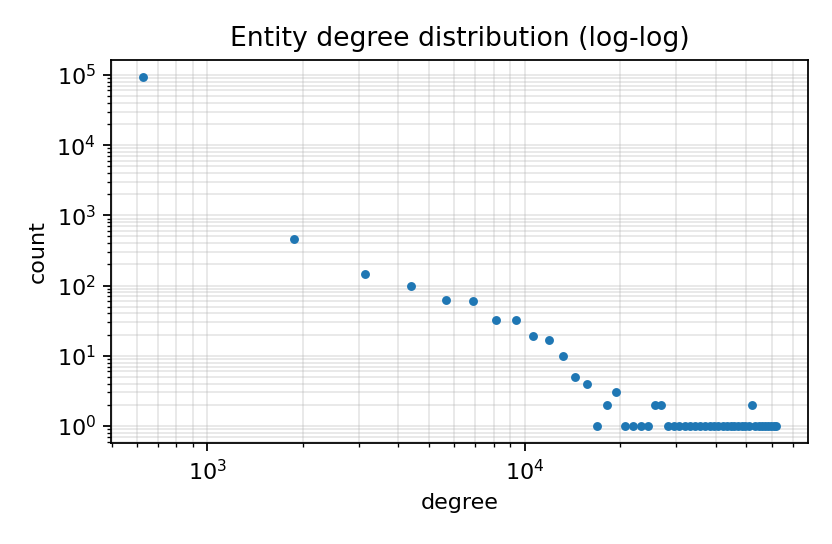
\includegraphics[width=\linewidth]{fig_degree_loglog.png}
    \end{column}
  \end{columns}
  \vspace{0.4em}
  Heavy-tailed degrees $\Rightarrow$ hubs make full 2-hop expansion unsafe.
\end{frame}

\begin{frame}{PySpark Pipeline}
  \begin{block}{Stages (then \texttt{spark.stop()})}
    \begin{enumerate}
      \item Ingest with explicit $(h,r,t)$ schema
      \item Clean nulls, duplicates, self-loops
      \item Profile degrees \& Bordes relation categories
      \item Dense IDs + inverse edges (102 message relations)
      \item Build int64 keys for filtered ranking
      \item Hand tensors to PyTorch; stop the JVM
    \end{enumerate}
  \end{block}
  Config: \texttt{local[*]}, Arrow, Kryo, 12\,GB driver, 8 partitions.
\end{frame}

\begin{frame}{Spark Scalability}
  \begin{columns}[T]
    \begin{column}{0.62\textwidth}
      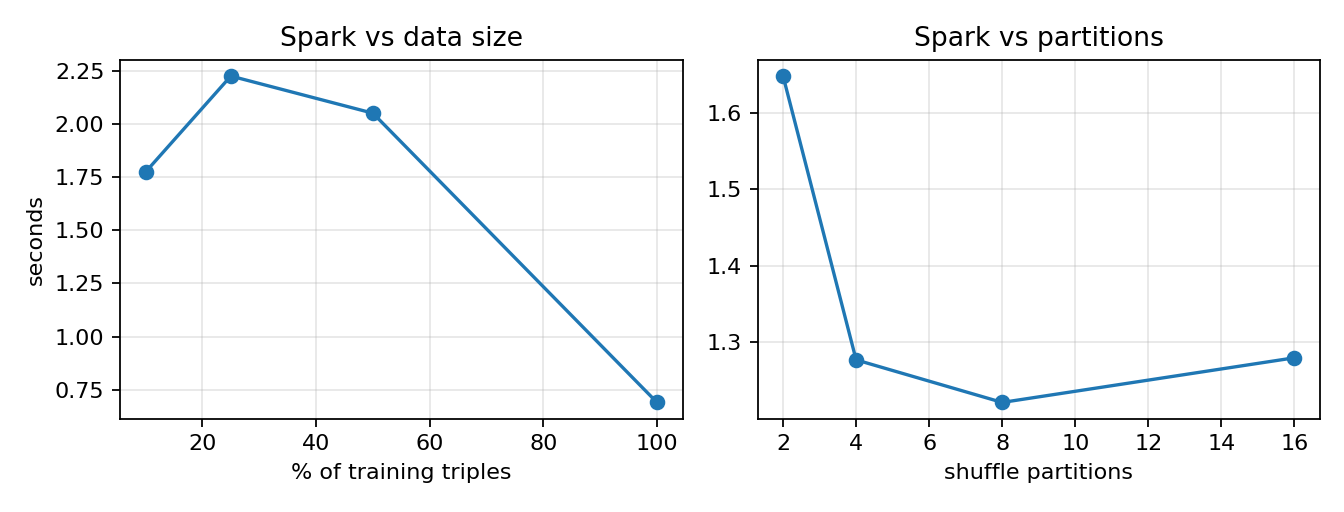
\includegraphics[width=\linewidth]{fig_spark_scale.png}
    \end{column}
    \begin{column}{0.36\textwidth}
      \begin{block}{Takeaways}
        \begin{itemize}
          \item ETL profiling in $\approx$1--2\,s
          \item 100\% fastest = cache hit
          \item Partitions 2$\to$16 are flat
        \end{itemize}
      \end{block}
    \end{column}
  \end{columns}
\end{frame}

% =====================================================================
\section{Models \& Training}

\begin{frame}{Models We Compare}
  \begin{columns}[T]
    \begin{column}{0.32\textwidth}
      \begin{block}{DistMult}
        $f=\sum_k h_k r_k t_k$\\
        Shared decoder + shallow baseline
      \end{block}
    \end{column}
    \begin{column}{0.32\textwidth}
      \begin{block}{R-GCN}
        Per-relation $W_r$\\
        Basis decomp.\ ($B{=}8$)\\
        2 layers, dim 128
      \end{block}
    \end{column}
    \begin{column}{0.32\textwidth}
      \begin{block}{CompGCN}
        $\phi(h,r)$: sub / mult / corr\\
        Direction-specific $W$\\
        Relation update each layer
      \end{block}
    \end{column}
  \end{columns}
  \vspace{0.6em}
  Extra shallow baselines (same budget): TransE and ComplEx.
\end{frame}

\begin{frame}{Making GNNs Fit on a 16\,GB T4}
  \begin{center}
  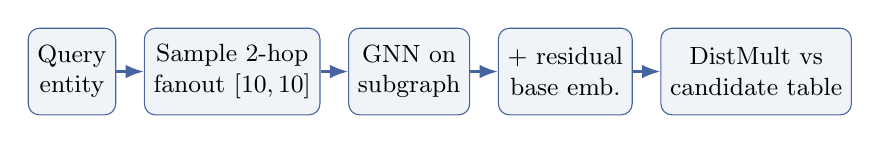
\begin{tikzpicture}[
      box/.style={draw=IITGBlue, rounded corners, align=center,
                   fill=IITGBlue!8, minimum height=1.1cm, font=\small},
      arr/.style={-{Latex}, thick, IITGBlue}]
    \node[box] (q) {Query\\entity};
    \node[box, right=0.35cm of q] (s) {Sample 2-hop\\fanout $[10,10]$};
    \node[box, right=0.35cm of s] (g) {GNN on\\subgraph};
    \node[box, right=0.35cm of g] (r) {$+$ residual\\base emb.};
    \node[box, right=0.35cm of r] (d) {DistMult vs\\candidate table};
    \draw[arr] (q)--(s); \draw[arr] (s)--(g);
    \draw[arr] (g)--(r); \draw[arr] (r)--(d);
  \end{tikzpicture}
  \end{center}
  \vspace{0.5em}
  \begin{itemize}
    \item Query-side encoding only; candidates from \texttt{model.ent}
    \item Mixed precision; CompGCN composition forced to float32
    \item OOM fallback: halve batch \& fanout
  \end{itemize}
\end{frame}

\begin{frame}{Training Recipe}
  \begin{columns}[T]
    \begin{column}{0.55\textwidth}
      \begin{block}{Design choices}
        \begin{itemize}
          \item Bidirectional: $(h,r,?)$ and $(?,r,t)$
          \item \textbf{Matched budget} for all 7 models
          \item Type-aware negatives (same entity type)
          \item Self-adversarial weighting (RotatE-style)
          \item Early stop on val.\ MRR (patience 5)
        \end{itemize}
      \end{block}
    \end{column}
    \begin{column}{0.43\textwidth}
      \begin{block}{T4 preset}
        \begin{tabular}{lr}
          Epochs $\times$ steps & $12\times 600$ \\
          Negatives / batch & 16 / 512 \\
          Dim / layers / bases & 128 / 2 / 8 \\
          Fanout & $[10,10]$ \\
          Wall clock & 1.76\,h \\
        \end{tabular}
      \end{block}
    \end{column}
  \end{columns}
\end{frame}

\begin{frame}{Two Evaluation Protocols}
  \begin{columns}[T]
    \begin{column}{0.48\textwidth}
      \begin{block}{Filtered candidates}
        \begin{itemize}
          \item True vs 500 random entities
          \item Other truths masked (Spark keys)
          \item Head + tail, 15{,}000 triples
          \item Used each validation epoch
        \end{itemize}
      \end{block}
    \end{column}
    \begin{column}{0.48\textwidth}
      \begin{block}{Official OGB}
        \begin{itemize}
          \item Type-constrained negatives
          \item 162{,}870 test triples
          \item Comparable to literature
          \item \textbf{Main reported metric}
        \end{itemize}
      \end{block}
    \end{column}
  \end{columns}
  \vspace{0.5em}
  \alert{Lesson:} OGB negatives are row-aligned; Spark reorders rows ---
  evaluate OGB on the original test order.
\end{frame}

% =====================================================================
\section{Results \& Lessons}

\begin{frame}{Main Result: Official OGB Evaluator}
  \begin{center}
  \small
  \begin{tabular}{lcccc}
    \toprule
    Model & MRR & H@1 & H@3 & H@10 \\
    \midrule
    DistMult & 0.325 & 0.224 & 0.364 & 0.526 \\
    R-GCN & 0.547 & 0.434 & 0.606 & 0.768 \\
    CompGCN-sub & 0.578 & 0.464 & 0.641 & 0.799 \\
    \textbf{CompGCN-mult} & \textbf{0.620} & \textbf{0.505} & \textbf{0.691} & \textbf{0.835} \\
    CompGCN-corr & 0.004 & 0.000 & 0.000 & 0.000 \\
    TransE & 0.270 & 0.165 & 0.305 & 0.490 \\
    ComplEx & 0.250 & 0.168 & 0.278 & 0.410 \\
    \bottomrule
  \end{tabular}
  \end{center}
  \vspace{0.5em}
  CompGCN-mult $>$ CompGCN-sub $>$ R-GCN $>$ TransE/ComplEx $>$ DistMult
\end{frame}

\begin{frame}{OGB Metrics (Visual)}
  \begin{center}
    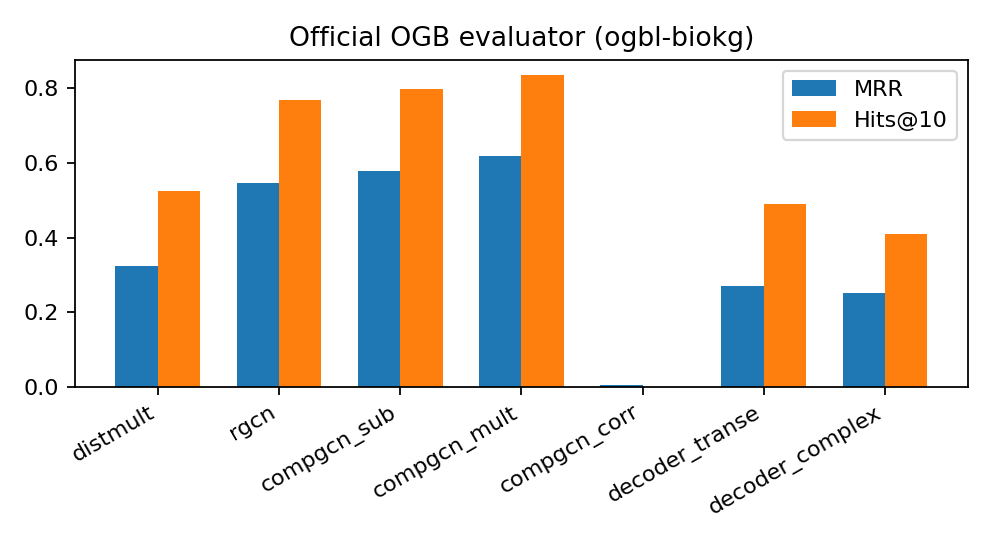
\includegraphics[width=0.92\linewidth]{fig_ogb_bars.png}
  \end{center}
\end{frame}

\begin{frame}{Second Protocol Agrees (500 Candidates)}
  \begin{columns}[T]
    \begin{column}{0.48\textwidth}
      \small
      \begin{tabular}{lccc}
        \toprule
        Model & MRR & H@10 & MR \\
        \midrule
        DistMult & 0.348 & 0.562 & 63.4 \\
        R-GCN & 0.549 & 0.798 & 13.5 \\
        CompGCN-sub & 0.576 & 0.828 & 11.6 \\
        \textbf{CompGCN-mult} & \textbf{0.631} & \textbf{0.867} & 9.5 \\
        CompGCN-corr & 0.002 & 0.000 & 485.1 \\
        TransE & 0.285 & 0.519 & 56.5 \\
        ComplEx & 0.275 & 0.448 & 110.6 \\
        \bottomrule
      \end{tabular}
    \end{column}
    \begin{column}{0.50\textwidth}
      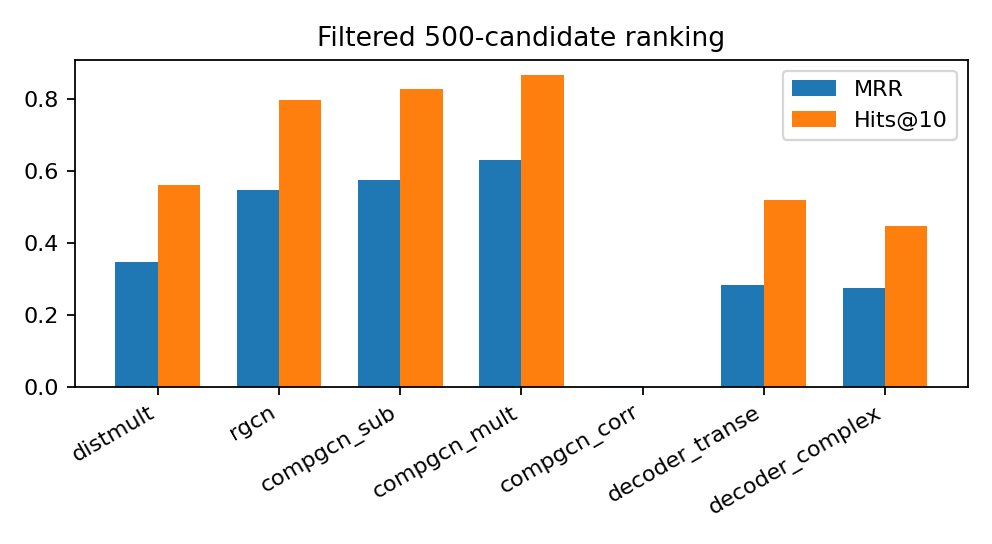
\includegraphics[width=\linewidth]{fig_main_bars.png}
    \end{column}
  \end{columns}
  \vspace{0.3em}
  Same ranking as OGB; matched budget removed the earlier DistMult artifact.
\end{frame}

\begin{frame}{Training Dynamics}
  \begin{center}
    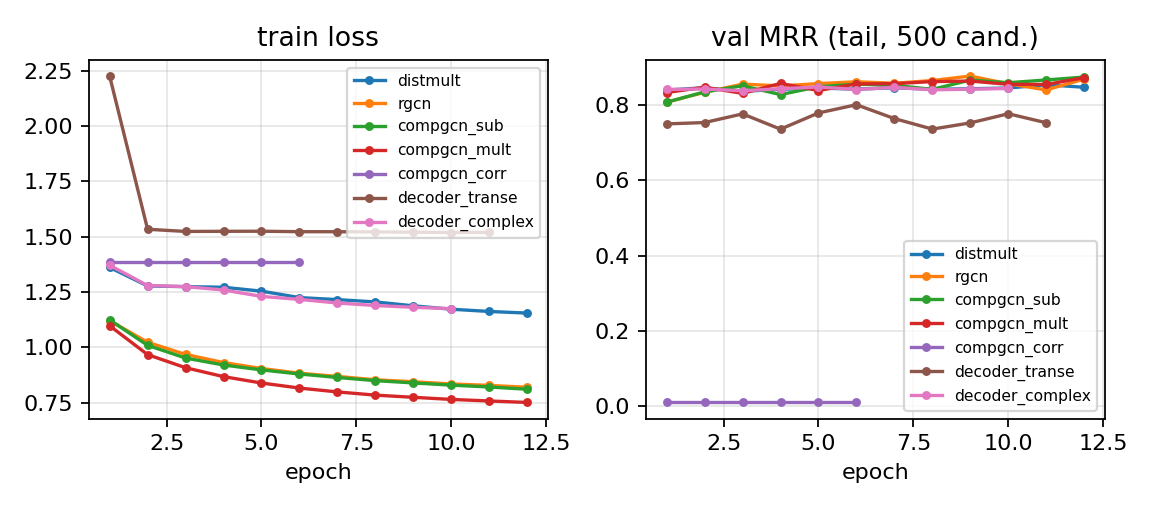
\includegraphics[width=\linewidth]{fig_train_curves.png}
  \end{center}
  Lowest loss: CompGCN-mult. CompGCN-corr collapses after epoch~1
  (early-stopped at epoch~6); all others run 12 epochs.
\end{frame}

\begin{frame}{R-GCN Ablations (Half Budget)}
  \begin{columns}[T]
    \begin{column}{0.62\textwidth}
      \small
      \begin{tabular}{lcccc}
        \toprule
        Setting & MRR & H@1 & H@10 & MR \\
        \midrule
        Base (128, L2, B8, n16) & 0.411 & 0.291 & 0.655 & 32.5 \\
        \textbf{1 layer} & \textbf{0.449} & \textbf{0.323} & 0.701 & 26.7 \\
        8 negatives & 0.332 & 0.213 & 0.582 & 48.5 \\
        4 bases & 0.395 & 0.270 & 0.644 & 34.0 \\
        dim 64 & 0.436 & 0.316 & 0.679 & 28.7 \\
        \bottomrule
      \end{tabular}
    \end{column}
    \begin{column}{0.36\textwidth}
      \begin{block}{Takeaways}
        \begin{itemize}
          \item 1 layer strongest
          \item 8 negatives hurts most
          \item dim 64 still competitive
        \end{itemize}
      \end{block}
    \end{column}
  \end{columns}
\end{frame}

\begin{frame}{Error Analysis: Rare Entities Are Hard}
  \begin{columns}[T]
    \begin{column}{0.48\textwidth}
      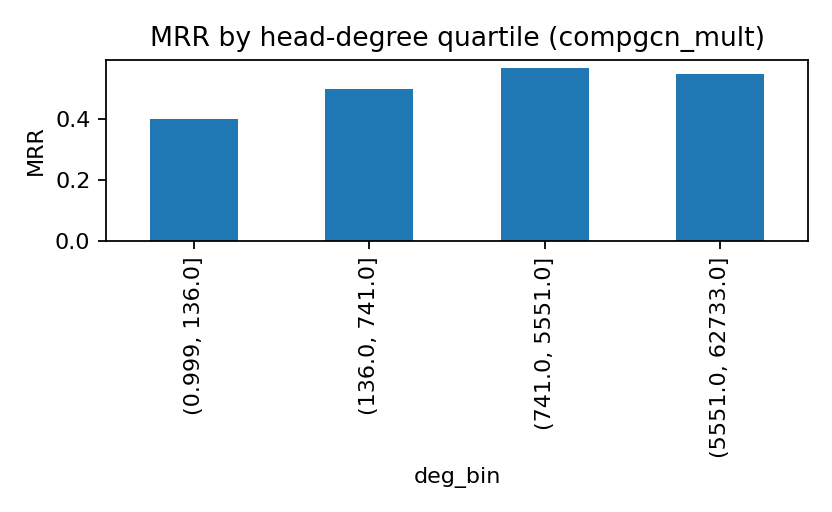
\includegraphics[width=\linewidth]{fig_mrr_by_degree.png}
    \end{column}
    \begin{column}{0.48\textwidth}
      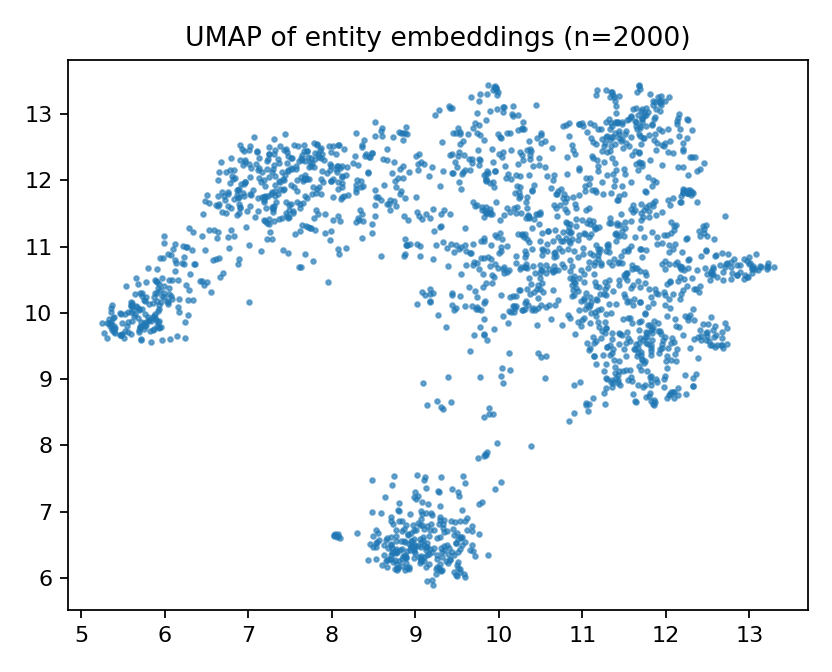
\includegraphics[width=\linewidth]{fig_umap_entities.png}
    \end{column}
  \end{columns}
  \vspace{0.3em}
  CompGCN-mult: MRR 0.401 (rarest quartile) vs 0.568 (best bin).
  All 51 relations are N--N $\Rightarrow$ relation-type breakdown uninformative.
\end{frame}

\begin{frame}{Engineering Lessons}
  \begin{itemize}
    \item \textbf{OGB misalignment:} Spark reordered test rows; evaluate on
          original OGB order.
    \item \textbf{Half-precision FFT:} CompGCN-corr broke under AMP;
          composition now float32.
    \item \textbf{Kernel deaths:} per-row negatives $\to$ millions of tensors;
          vectorize by entity type.
    \item \textbf{CUDA~13 installs:} compiling \texttt{torch-scatter} kills
          the kernel; binary wheels only.
  \end{itemize}
\end{frame}

\begin{frame}{Conclusion}
  \begin{columns}[T]
    \begin{column}{0.32\textwidth}
      \begin{block}{Results}
        \begin{itemize}
          \item Spark ETL in seconds
          \item Sampled GNNs fit a T4
          \item CompGCN-mult best (OGB MRR 0.620)
          \item GNNs $\gg$ shallow at equal budget
        \end{itemize}
      \end{block}
    \end{column}
    \begin{column}{0.32\textwidth}
      \begin{block}{Limits}
        \begin{itemize}
          \item Below published long-schedule SOTA
          \item Candidates not GNN-encoded
          \item CompGCN-corr unstable
          \item Spark on one node
        \end{itemize}
      \end{block}
    \end{column}
    \begin{column}{0.32\textwidth}
      \begin{block}{Future}
        \begin{itemize}
          \item Encode both sides
          \item ConvE decoder
          \item Stabilize corr
          \item Multi-node Spark / Wikidata5M
        \end{itemize}
      \end{block}
    \end{column}
  \end{columns}
\end{frame}

\begin{frame}{Thank You --- Questions?}
  \begin{center}
    {\Large Knowledge Graph Completion with R-GCN / CompGCN}\\[1.2em]
    Code, notebook, results and report:\\[0.4em]
    {\small\url{https://github.com/Charanponaganti/Knowledge-Graph-Completion-with-R-GCN-CompGCN}}\\[1.5em]
    Charan Ponaganti \quad M Charan \quad Lalit Deshmane
  \end{center}
\end{frame}

\end{document}
